\documentclass{exam}
\usepackage{mainExam}

\title{Contrôle : généralités sur les fonctions}
\date{2 Mai 2025}
\author{Seconde 9}

\begin{document}
\maketitle
\instructions{Interdite}
\begin{questions}
\titledquestion{Etude de fonction}[6]
On étudie la fonction $f$ dont la courbe représentative est donnée ci-après :
\begin{center}
\begin{tikzpicture}
\repereclassique{-4.25}{-4.25}{4.25}{4.25}{0.5};
\draw[thick] (-4,0) parabola bend (-2.5,3) (-1,2);
\draw[thick] (-1,2) parabola bend (0.5,-1.5) (1.5,0);
\draw[thick] (1.5,0) parabola bend (2,1) (3,0);
\draw[thick] (3,0) parabola bend (3.5,-2) (4,-0.5);
\draw (-4,0) node {$\bullet$};
\draw (4,-0.5) node {$\bullet$};
\end{tikzpicture}
\end{center}
\begin{parts}
\part[1] Résoudre les équations suivantes. On justifiera ses résultats en faisant apparaître des traits de construction sur la figure.
\begin{subparts}
\subpart $f(x) = 2$
\subpart $f(x) = -3$
\end{subparts}
\part[1] Résoudre l'inéquation $f(x) \geq 0$. On justifiera ses résultats en faisant apparaître des traits de construction sur la figure.
\part[2] Compléter le tableau de variation de cette fonction.
\begin{center}
\begin{tikzpicture}
\tkzTabInit{$x$ / 1, Variations de $f$ / 3}{,,,,}
\end{tikzpicture}
\end{center}
\part[2] En déduire le maximum et le minimum de $f$.
\end{parts}
\newpage
\titledquestion{Physique}[4]
Deux pots de fleurs tombent d'un balcon. L'un contient un cactus et l'autre des roses. Le voisin d'en face observe la chute. 
\begin{itemize}
\item On pose $c(t)$ la hauteur par rapport au sol (en \unit{\meter}) du pot contenant le cactus à l'instant $t$. 
\item On pose $r(t)$ la hauteur par rapport au sol (en \unit{\meter}) du pot contenant les roses à l'instant $t$. 
\end{itemize}
Le temps $t$ est donné en secondes.

Les courbes représentatives $\mathcal{C}_c$ et $\mathcal{C}_r$ sont données ci-après.
\begin{center}
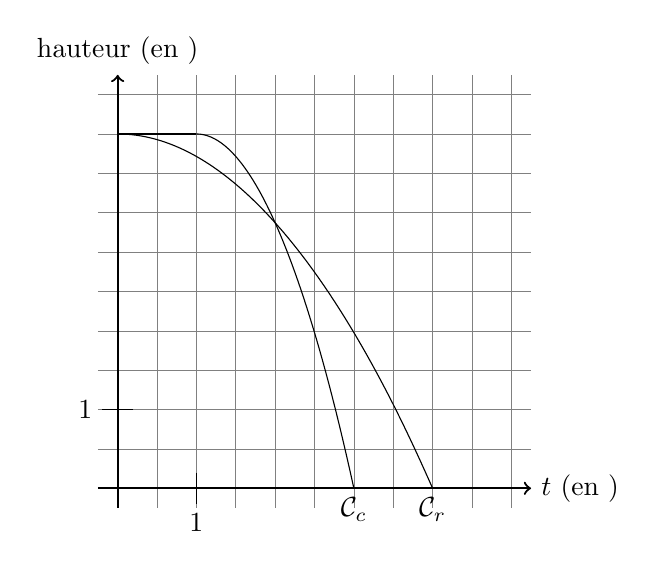
\begin{tikzpicture}
\draw[help lines] (-0.25,-0.25) grid[step=0.5] (5.25,5.25);
\draw[thick,->] (-0.25,0) -- (5.25,0) node[right] {$t$ (en \unit{\second})};       
\draw[thick,->] (0,-0.25) -- (0,5.25) node[above] {hauteur (en \unit{\meter})};
\draw (0.2,1) -- (-0.2,1) node[left] {$1$};
\draw (1,0.2) -- (1,-0.2) node[below] {$1$};

\draw (0,4.5) -- (1,4.5);
\draw (1,4.5) parabola (3,0) node[below] {$\mathcal{C}_c$};
\draw (0,4.5) parabola (4,0) node[below] {$\mathcal{C}_r$};
\end{tikzpicture}
\end{center}

Répondre aux questions suivantes, en justifiant chacune des réponses.
\begin{parts}
\part[1] Quelle est la hauteur du balcon ?
\part[1] À partir de quels instants chacune des plantes a commencé à tomber ?
\part[1] Quelle plante a touché le sol en premier ?
\part[1] À quels instants les pots étaient-ils à la même hauteur ?
\end{parts}
\vspace*{0.5cm}
\titledquestion{Géométrie}[8]
Le quadrilatère $ABCD$ est un rectangle vérifiant $AB = \qty{10}{\centi\meter}$ et $AD = \qty{6}{\centi\meter}$. Soit $M$ un point quelconque du segment $[AB]$; $N$ un point quelconque du segment $[BC]$; $P$ un point quelconque du segment $[CD]$ et $Q$ un point quelconque du segment $[AD]$, tels que $AM = BN = CP = DQ$. On pose $x$ la longueur $AM$.
\begin{center}
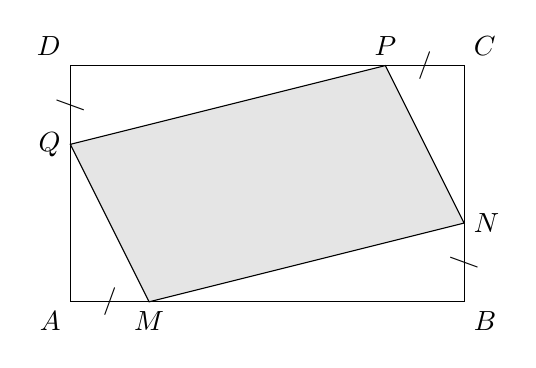
\begin{tikzpicture}
\draw (0,0) node[below left] {$A$} -- (5,0) node[below right] {$B$} -- (5,3) node[above right] {$C$} -- (0,3) node[above left] {$D$} -- cycle;
\fill[color=gray!20] (1,0) node[below] {$M$} -- (5,1) node[right] {$N$} -- (4,3) node[above] {$P$} -- (0,2) node[left] {$Q$} -- cycle;
\draw (1,0) node[below] {$M$} -- (5,1) node[right] {$N$} -- (4,3) node[above] {$P$} -- (0,2) node[left] {$Q$} -- cycle;

\draw (0,0) -- (1,0) node[midway] {$\slash$};
\draw (5,0) -- (5,1) node[midway,sloped] {$\slash$};
\draw (5,3) -- (4,3) node[midway,sloped] {$\slash$};
\draw (0,3) -- (0,2) node[midway,sloped] {$\slash$};
\end{tikzpicture}
\end{center}
On pose $f(x)$ l'aire du quadrilatère $MNPQ$.
\begin{parts}
\part[1] Compléter la figure en précisant les segments de longueur $x$ dans cette exemple.
\part[1] Justifier que $x$ est dans l'intervalle $[0;6]$.
\part[2] En considérant que l'aire de $MNPQ$ par rapport à l'aire de $ABCD$, montrer que l'expression de $f(x)$ en fonction de $x$ est donnée par :
\begin{equation*}
f(x) = 60 - x(10 - x) - x(6-x)
\end{equation*}
\part[2] En déduire que pour tout $x \in [0;6]$ $f(x) = 2(x-4)^2+28$.
\part[2] À l'aide de la courbe représentative de $g$ vérifiant $g(x) = 2(x-4)^2+28$ pour tout $x \in [0;6]$, en déduire pour quelle valeur de $x$ l'aire de $MNPQ$ est minimale.
\begin{center}
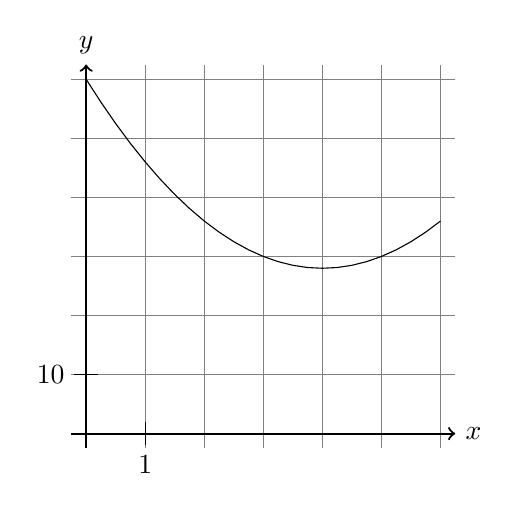
\begin{tikzpicture}[scale=0.75]
\draw[help lines] (-0.25,-0.25) grid (6.25,6.25);
\draw[thick,->] (-0.25,0) -- (6.25,0) node[right] {$x$};       
\draw[thick,->] (0,-0.25) -- (0,6.25) node[above] {$y$};
\draw (0.2,1) -- (-0.2,1) node[left] {$10$};
\draw (1,0.2) -- (1,-0.2) node[below] {$1$};

\draw [domain=0:6] plot (\x, {(\x-4)^2/5 + 28/10});
\end{tikzpicture}
\end{center}
\end{parts}
\vspace*{0.5cm}
\titledquestion{Dessin}[2]
Dessiner la courbe représentative d'une fonction vérifiant tous les critères suivants :
\begin{itemize}
\item La fonction est définie sur $[0;7]$;
\item $f(3) = 2$;
\item $f$ admet exactement trois antécédents à $-1$;
\item $f$ est croissante sur $[1;2]$;
\item $f$ admet $4$ comme maximum;
\item $f$ atteint son minimum en $6$.
\end{itemize}
\end{questions}
\end{document}